\documentclass{standalone}
\usepackage[dvipsnames]{xcolor}
\usepackage{upgreek}
\usepackage{filecontents,pgfplots}
\usetikzlibrary{patterns}
\begin{document}
\pgfplotsset{
    standard/.style={
  axis x line*=bottom,
  axis y line*=right,
        axis x line shift=0.1,
        enlargelimits=false
    }
}
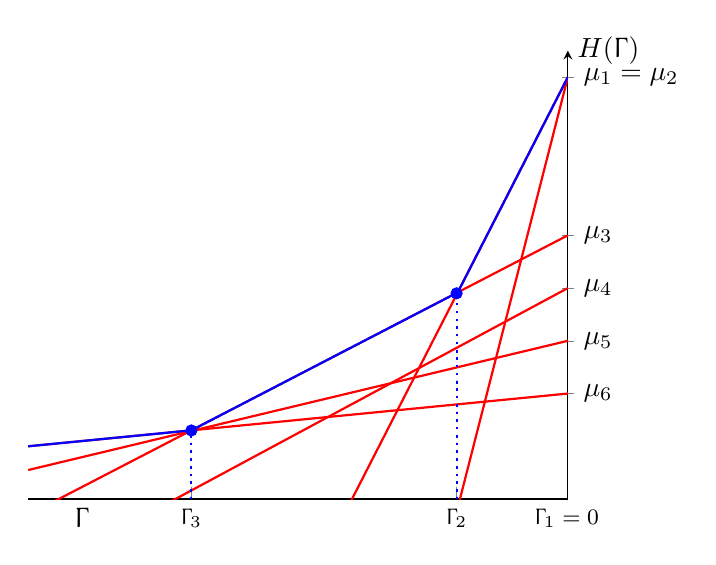
\begin{tikzpicture}[scale=1.]
\begin{axis}[xmin=-5,xmax=0,ymin=-1,ymax=3.25,
  axis x line*=bottom,
    axis y line=right,
      xlabel={$\Upgamma$}, 
    ylabel={$H(\Upgamma)$} , 
    ylabel style={rotate=-90},
            xtick={-3.4883,-1.0309,-0.01},
            xticklabels={{\footnotesize${\Upgamma}_{3}$},{\footnotesize${\Upgamma}_{2}$},{\footnotesize${\Upgamma}_1=0$}},
        ytick={3,1.5,1,0.5,0},
        yticklabels={$\mu_1=\mu_2$,$\mu_3$,$\mu_4$,$\mu_5$,$\mu_6$},
            every axis y label/.append style={at=(ticklabel* cs:1)},
            every axis x label/.append style={at=(ticklabel* cs:.1)},
            y tick label style={right},
                    ]
         %\addplot[white,pattern color = red, pattern = north east lines,opacity=.5] coordinates {(1,0) (2 ,-1)  (3,-1.5) (3,3) (-1, 4) (1,0)};
  \addplot[thick, red,domain=-5:0, samples=100]{0.5+.245*x};
    \addplot[thick, red,domain=-5:0, samples=100]{0+.1*x};
\addplot [thick,red,domain=-5:0, samples=100]{3+2*x};
\addplot [thick,red,domain=-5:0, samples=100]{3+4*x};
  \addplot [thick,red,domain=-5:0, samples=100]{1.5+.53*x};
    \addplot [thick,red,domain=-5:0, samples=100]{1+.55*x};
    
    \addplot [thick,blue,dotted,domain=-1:.95, samples=100](-1.0309,x);
    \addplot [thick,blue,dotted,domain=-1:-0.35, samples=100](-3.4883,x);
    
    
 \addplot [thick,blue,domain=-5:-3.4883, samples=100]{0+0.1*x};
 \addplot [thick,blue,domain=-3.4883:-1.0309, samples=100]{1.5+.53*x};
 \addplot [thick,blue,domain=-1.0309:0, samples=100]{3+2*x};

    
%\addplot[blue,thick] (cs:(0,0.5))  (cs:(-1.0309,2.05));

\addplot[only marks, mark=*, blue] table {
   -3.4883 -0.35
  };
  \addplot[only marks, mark=*, blue] table {
  -1.0309  .95
  };
  \addplot[only marks, mark=diamond*, blue] table {
  2  -1
  };
  \node [rotate=48] at (axis cs:  .7,  .59) {$$};
\end{axis}
\end{tikzpicture}

\end{document}